%
% intro.tex -- Einleitung zum Thema
%
% !TEX root = ../../buch.tex
% !TEX encoding = UTF-8
%
\section{Einleitung}

Wirbelringe sind ein interessantes Naturphänomen, welchem man schneller begegnet als man denkt. 
In diesem Paper schauen wir uns Wirbelringe etwas genauer an und begründen einige Eigenschaften. 
Des Weiteren untersuchen wir eine weitverbreitete praktische (ungewollte) Anwendung und dessen Auswirkung. 
Zuletzt formulieren wir ein Modell, womit man zumindest angenähert selbst gezielt Wirbelringe berechnen und erzeugen kann.

In diesem Paper werden, wo nicht anders angegeben, nur ideale Fluide betrachtet.
John von Neumann soll über die Theorie der idealen Fluide gesagt haben\cite{Wirbelringe:feynman1964lectures}: 
\begin{quote}
    The theory of inviscid fluids is the study of «dry water».
\end{quote}
Für das Verständnis von Wirbelringen ist sie aber ausreichend.

\subsection{Wirbel}

\begin{figure}
\centering
\begin{tikzpicture}
\clip (-6.3,-2.7) rectangle (6.3,2.7);
\node at (-0.07,-0.07) {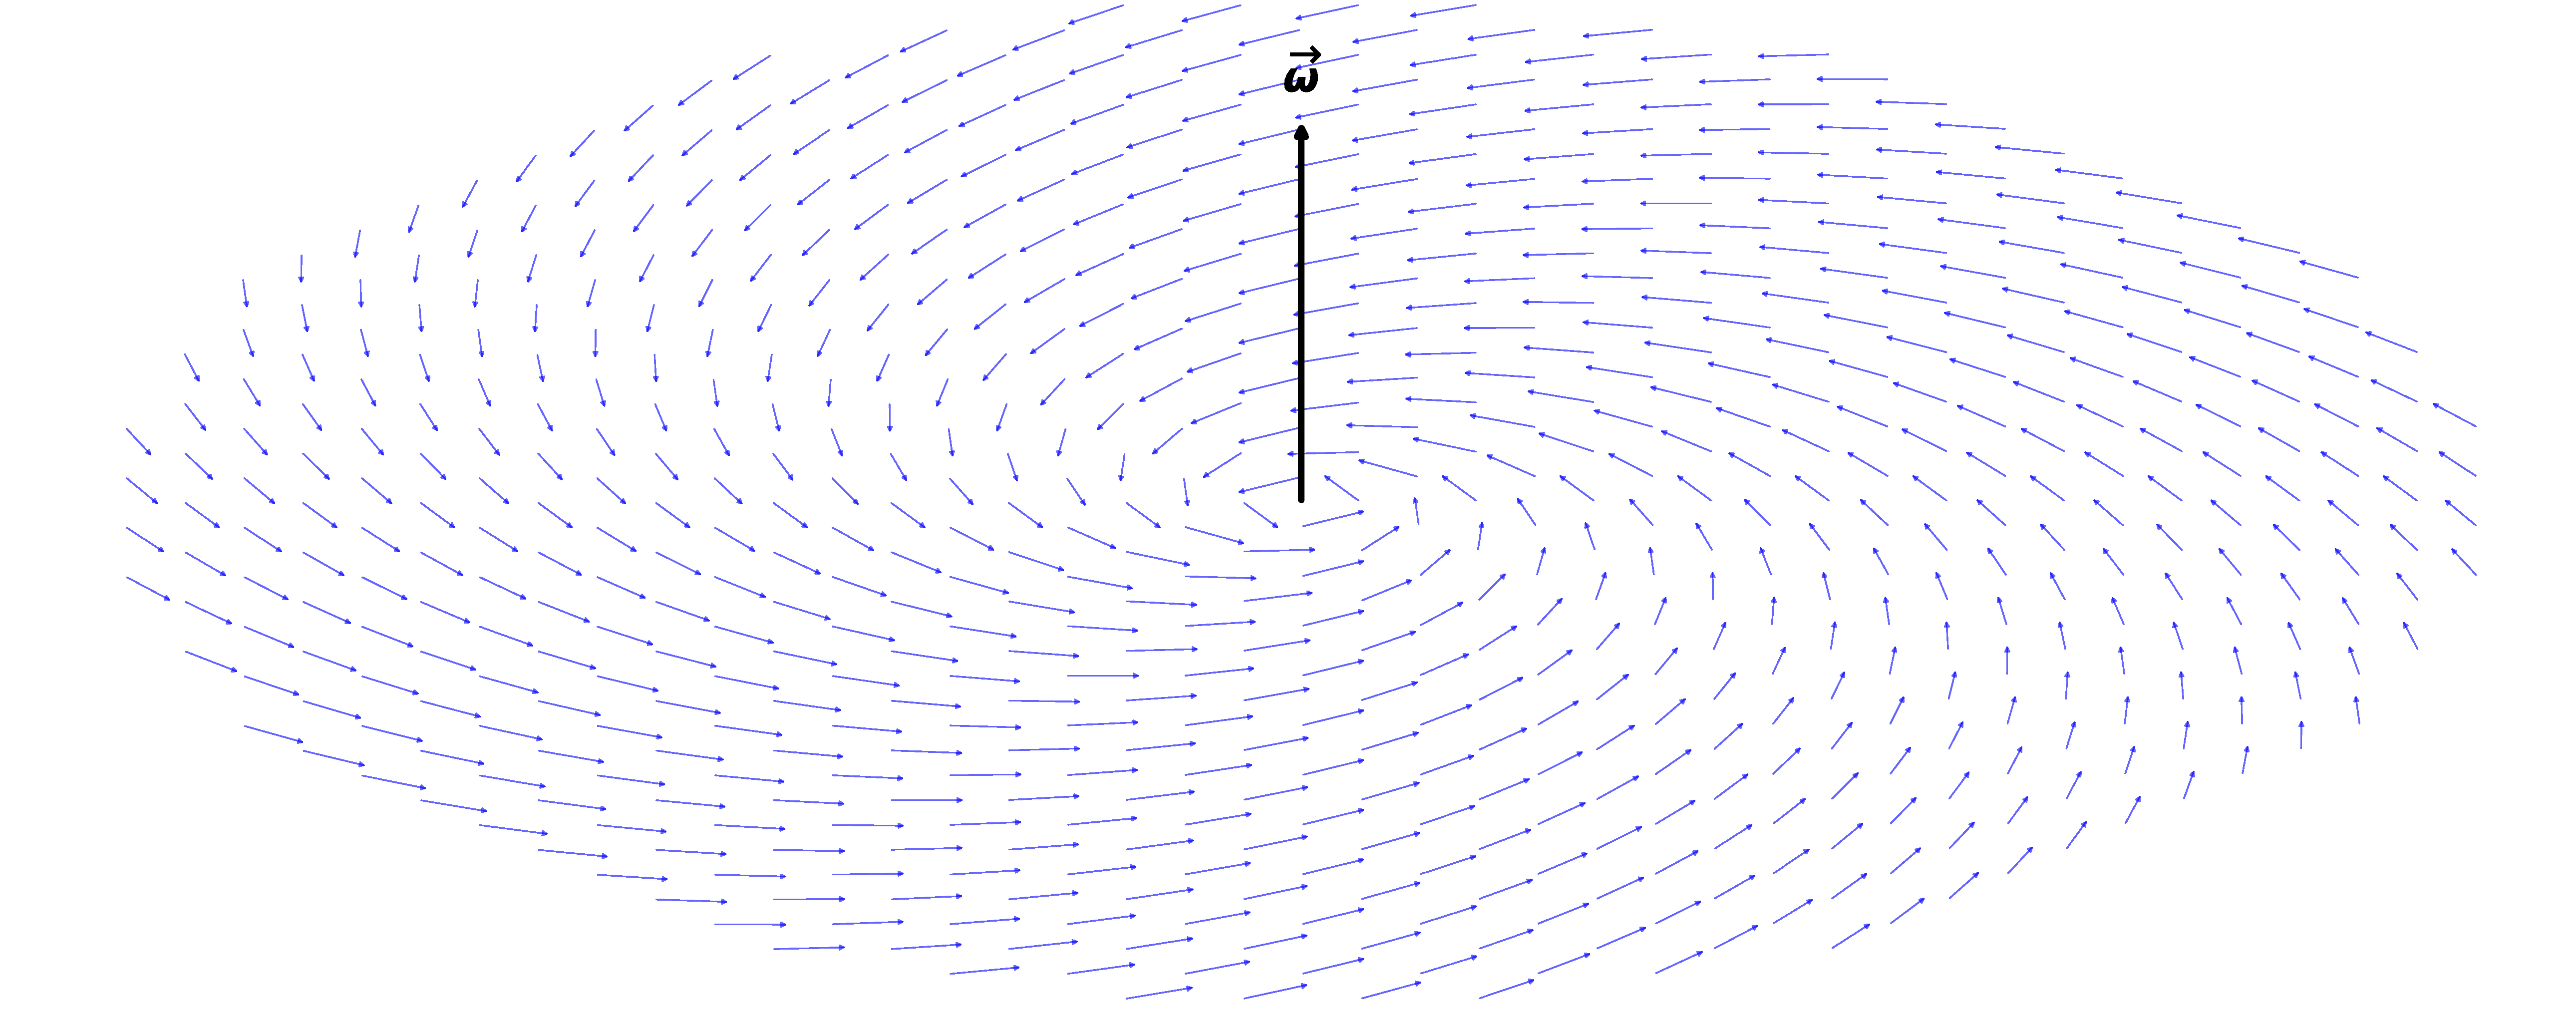
\includegraphics[width=1.08\textwidth]{papers/wirbelringe/fig/flacher_wirbel.pdf}};
%\draw[color=red] (-6.3,-2.7) rectangle (6.3,2.7);
\end{tikzpicture}
\caption{Darstellung eines 2-dimensionalen Wirbels mit Wirbelvektor
\(\vec{\omega}\).
\label{Wirbelringe:fig:flacher_wirbel}}
\end{figure}


Für die Betrachtung von Wirbelringen starten wir zunächst mit einzelnen Wirbeln.
Ein Wirbel ist eine Formation von Teilchen, welche um einen Mittelpunkt rotieren.
In Abbildung \ref{Wirbelringe:fig:flacher_wirbel} ist ein Wirbel abgebildet.
Die eingezeichneten Pfeile stellen die Geschwindigkeitsvektoren \( \vec{v} \) der Teilchen, welche Teil des Wirbels sind, dar.
Nicht explizit eingezeichnet sind die Bahnen, auf welchen sich die Teilchen bewegen.
Die Bahnen bilden konzentrische Kreise.
Auch ist in der Abbildung \ref{Wirbelringe:fig:flacher_wirbel} der Wirbelstärkevektor \(\vec{\omega}\) eingezeichnet.
Wir kommen später genauer auf \(\vec{\omega}\) zu sprechen.

\subsubsection*{Wirbellinien\label{Wirbelringe:Wirbellinien}}

Um Wirbel besser zu beschreiben, führen wir hier den Begriff {\em Wirbellinie} ein.
Wirbellinien sind die „Mittelachsen“ von Wirbeln. 
Um diese Achse rotieren die Teile, welche Teil eines Wirbels sind. 
Diese hat an sich kein Volumen, allerdings kann es sein, dass Teilchen auf dieser Achse zu liegen kommen. 
\(\vec{\omega}\) steht tangential zu dieser Wirbellinie.  
In der Praxis ist eine Wirbellinie nicht gerade, sondern gekrümmt oder sogar spiralenähnlich. 
Des Weiteren ist eine sehr wichtige Eigenschaft, dass Wirbellinien nur auf einer Grenzfläche enden können, 
wie wir in Abschnitt \ref{Wirbelringe:Grenzflaechen} sehen werden.

\subsection{Stabilität}

Um die Stabilität von Wirbeln zu beurteilen, können wir betrachten, wie sich die Menge an Teilchen verhält --- ob diese wächst oder schrumpft. 
Wir betrachten also die Divergenz der Teilchen, die Teil eines Wirbels sind.
Die Kontinuitätsgleichung 
\[
\frac{\partial \rho}{\partial t}
+
\operatorname{div}\vec{\jmath}
=
0
\]
aus Abschnitt \ref{buch:zusammenhang:erhaltungssatz:subsection:kontinuitaetsgleichung} besagt: Wenn mehr herausfliesst, als hineinfliessen kann --- was einer positiven Divergenz entspricht ---, dann muss die Dichte \(\rho\) abnehmen.

In unserem Fall ist \(\vec{\jmath}\) die Rotation eines Vektorfeldes z.B. \(\operatorname{rot}(\vec{A})\).
Um nun zu beurteilen, ob ein Wirbel stabil ist, können wir die Divergenz der Rotation eines Vektorfeldes betrachten.
Denn Stabilität bedeutet, dass die Anzahl der Teilchen konstant bleibt, also die Dichte gleich bleibt.
Somit stellt sich die Frage, ob

\begin{equation*}
\operatorname{div} \big( \operatorname{rot} ( \vec{A} ) \big)
\stackrel{?}{=}
0,
\end{equation*}
wobei wir für \(\vec{A}\) das Vektorfeld aus Abbildung \ref{Wirbelringe:fig:flacher_wirbel} verwenden.
Nehmen wir an, dass \(\vec{A}\) zweimal stetig differenzierbar ist, so können wir
\begin{align*}
\operatorname{div} ( \operatorname{rot} ( \vec{A} ) )
&=
\operatorname{div}      
    \begin{pmatrix} 
        \frac{\partial A_z}{\partial y} - \frac{\partial A_y}{\partial z} \\ 
        \frac{\partial A_x}{\partial z} - \frac{\partial A_z}{\partial x} \\ 
        \frac{\partial A_y}{\partial x} - \frac{\partial A_x}{\partial y} \\ 
    \end{pmatrix} \\
\intertext{setzen. Mit der Definition der Divergenz ergibt sich}
&=
\frac{\partial^2 A_z}{\partial x\, \partial y} - \frac{\partial^2 A_y}{\partial x\, \partial z} + 
\frac{\partial^2 A_x}{\partial y\, \partial z} - \frac{\partial^2 A_z}{\partial y\, \partial x} +
\frac{\partial^2 A_y}{\partial z\, \partial x} - \frac{\partial^2 A_x}{\partial z\, \partial y}
.\\
\intertext{Der Satz von Schwarz besagt, dass es nicht auf die Reihenfolge der Ableitungen ankommt. Somit kann man sie paarweise anordnen:}\\
&=
\frac{\partial^2 A_z}{\partial x\, \partial y} - \frac{\partial^2 A_z}{\partial y\, \partial x} + 
\frac{\partial^2 A_x}{\partial y\, \partial z} - \frac{\partial^2 A_x}{\partial z\, \partial y} +
\frac{\partial^2 A_y}{\partial z\, \partial x} - \frac{\partial^2 A_y}{\partial x\, \partial z}.
\\
\intertext{Da sich die Ableitungen dadurch aufheben, folgt}
&=
\overbrace{\frac{\partial^2 A_z}{\partial x\, \partial y} - \frac{\partial^2 A_z}{\partial x\, \partial y}}^0 + 
\overbrace{\frac{\partial^2 A_x}{\partial y\, \partial z} - \frac{\partial^2 A_x}{\partial y\, \partial z}}^0 +
\overbrace{\frac{\partial^2 A_y}{\partial x\, \partial z} - \frac{\partial^2 A_y}{\partial x\, \partial z}}^0
\\
&=
0.
\end{align*}
Somit gilt 
\begin{equation} 
    \label{Wirbelringe:eq:wIdent} 
    \operatorname{div} \big( \operatorname{rot} ( \vec{A} ) \big) 
    = 
    0. 
\end{equation} 
In einem idealisierten, reibungsfreien Wirbelfeld bleibt daher die Dichte konstant, was in diesem Modell einer stabilen Wirbelstruktur entspricht.

\subsection{Vom Wirbel zum Wirbelring}

Um aus Wirbeln ein Wirbelring zu machen, brauchen wir noch eine Definition.

\subsubsection*{Wirbelfäden}

Ein {\em Wirbelfaden} ist ein Zylinder, welcher eine Wirbellinie als Zentrum hat.
Schneidet man nun diesen Zylinder senkrecht zu der Wirbellinie, ergibt sich ein einzelner Wirbel.
Wirbelfäden werden auch {\em Wirbelröhren} genannt.

Um aus einem Wirbelfaden einen Wirbelring zu machen, schliessen wir die offenen Enden (wir betrachten später, wie man mit diesen umzugehen hat) zusammen.
Die Wirbellinie formt ein Kreis.
Jetzt ist es ein Wirbelring. 
Solch ein Wirbelring ist in Abbildung \ref{Wirbelringe:fig:generell} dargestellt.

\input{papers/wirbelringe/images/wirbelring.png}
